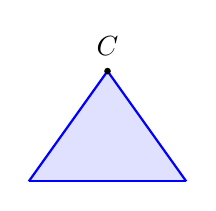
\begin{tikzpicture}[scale=1]
  \coordinate (A) at (-1,0);
  \coordinate (B) at (1,0);
  \coordinate (C) at (0,1.4);
  \fill[blue!12] (A)--(B)--(C)--cycle;
  \draw[blue,line width=0.8pt] (A)--(B);
  \draw[blue,line width=0.8pt] (B)--(C);
  \draw[blue,line width=0.8pt] (C)--(A);
  \fill (C) circle (1.2pt);
  \node[above=2pt] at (C) {$C$};
\end{tikzpicture}
